\documentclass[a4paper,14pt]{extarticle}
\usepackage{../../tex-shared/report-layout}

\renewcommand{\mylabnumber}{1}
\renewcommand{\mylabtitle}{Исследование методов администрирования 1С: Предприятие 8}
\renewcommand{\mysubject}{Платформа 1С}
\renewcommand{\mylecturer}{Кудашев В.С.}

\begin{document}
\begin{titlepage}
    
    \thispagestyle{empty}
    
    \begin{center}
        
        Министерство науки и Высшего образования Российской Федерации \\
        Севастопольский государственный университет \\
        Кафедра ИС
        
        \vfill

        Отчет \\
        по лабораторной работе №\mylabnumber \\
        \enquote{\mylabtitle} \\
        по дисциплине \\
        \enquote{\MakeTextUppercase{\mysubject}}

    \end{center}

    \vspace{1cm}

    \noindent\hspace{7.5cm} Выполнил студент группы ИС/б-17-2-о \\
    \null\hspace{7.5cm} Горбенко К. Н. \\
    \null\hspace{7.5cm} Проверил \\
    \null\hspace{7.5cm} \mylecturer

    \vfill

    \begin{center}
        Севастополь \\
        \the\year{}
    \end{center}

\end{titlepage}

\section{Цель работы}
\begin{enumerate}
    \item Ознакомление с системой автоматизации экономической и организационной
          деятельности предприятия – «1С:Предприятие 8»;
    \item Изучение основных средств администрирования «1С:Предприятие 8».
\end{enumerate}

\section{Задание на работу}
\begin{enumerate}
    \item Ознакомится с теоретическим материалом в методических указаниях.
    \item Произвести добавление новой информационной базы. Расположение исходной
          базы данных уточнить у преподавателя.
    \item Создать подсистемы справочников и документов.
    \item Создать роли. Для каждой роли описать набор прав на выполнение
          действий над объектами базы данных и над всей конфигурацией в целом.
    \item Создать пользователей информационной базы с настройками согласно
          варианту. Поставить в соответствие роли, которые существуют в
          конфигурации базы данных.
    \item Запустить систему в режиме предприятия под каждым из пользователей,
          проверить работу прав доступа. Проконтролировать список активных
          пользователей.
    \item Ознакомиться с текущей настройкой журнала регистрации. Установить
          режим «Регистрировать ошибки, предупреждения, информацию, примечания». В
          режиме предприятия произвести какие-либо действия (создать новый документ,
          изменить существующие документы). Проконтролировать регистрацию в журнале.
    \item Произвести выгрузку информационной базы, используя встроенные средства.
    \item Создать пустую информационную базу. Восстановить данные из резервной
          копии (выгрузки, сделанной в предыдущем пункте).
    \item Произвести тестирование и исправление информационной базы.
    \item Выполнить запуск утилиты восстановления файловой базы данных и
          выполнить проверку файла базы данных.
    \item Сформулировать выводы.
    \item Оформить отчет.
\end{enumerate}
\pagebreak

Вариант № 1:
\begin{figure}[H]
    \centering
    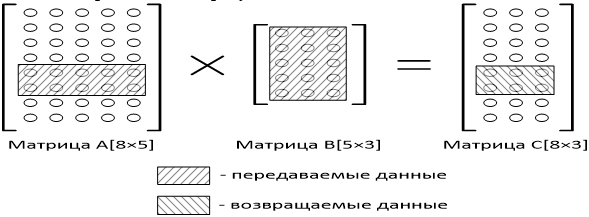
\includegraphics[width=\linewidth]{task}
    \caption{Задание по варианту}
    \label{fig:task}
\end{figure}

\section{Ход работы}
Создадим информационную базу \enquote{Управление прайс-листами}, добавим
подсистемы \enquote{Товары, Ценообразование}, \enquote{Ценовая политика}.
Результат представлен на рисунках \ref{fig:infobase} и \ref{fig:subsystems}.
\begin{figure}[H]
    \centering
    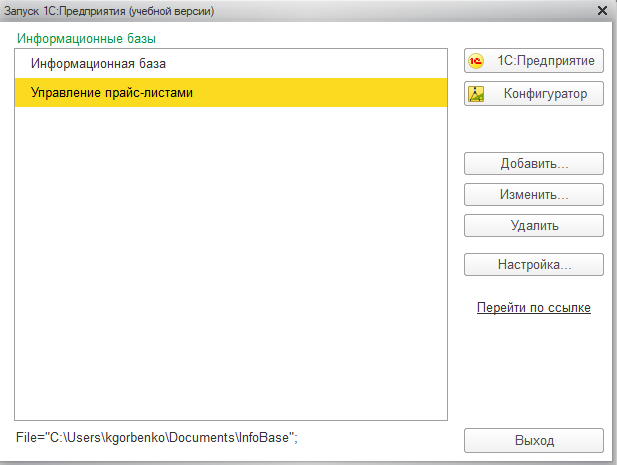
\includegraphics[width=0.6\linewidth]{infobase}
    \caption{Созданная информационная база}
    \label{fig:infobase}
\end{figure}
\begin{figure}[H]
    \centering
    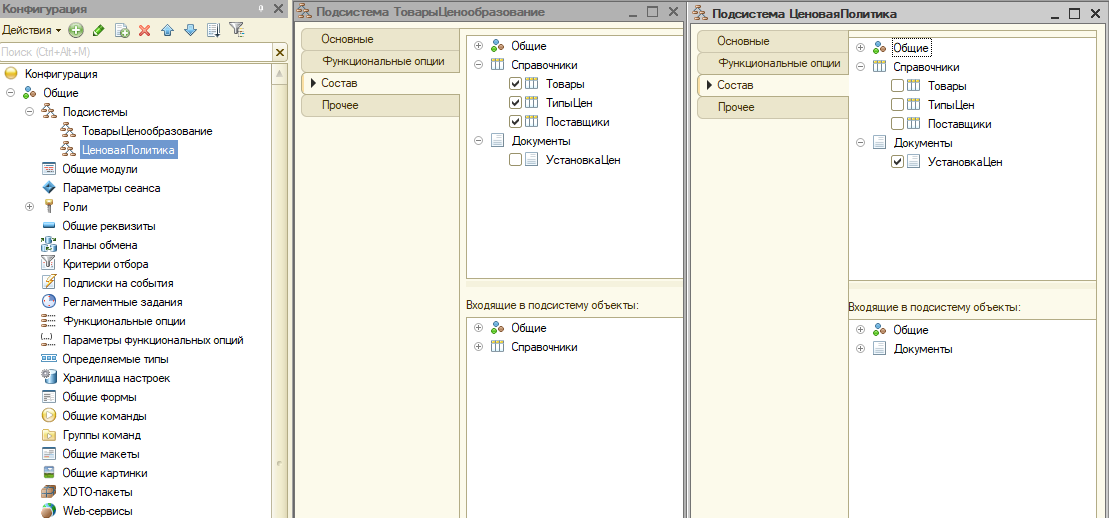
\includegraphics[width=\linewidth]{subsystems}
    \caption{Состав подсистем}
    \label{fig:subsystems}
\end{figure}

Создадим роли \enquote{Администратор} и \enquote{Менеджер по закупкам}.
Администратору доступен конфигуратор и все операции над данными в справочниках и
документах. Менеджеру по закупкам доступны операции просмотра в подсистеме
\enquote{Ценовая политика} и операции добавления и редактирования данных в
подсистеме \enquote{Товары, ценообразование}. Результат представлен на рисунке
\ref{fig:roles}.
\begin{figure}[H]
    \centering
    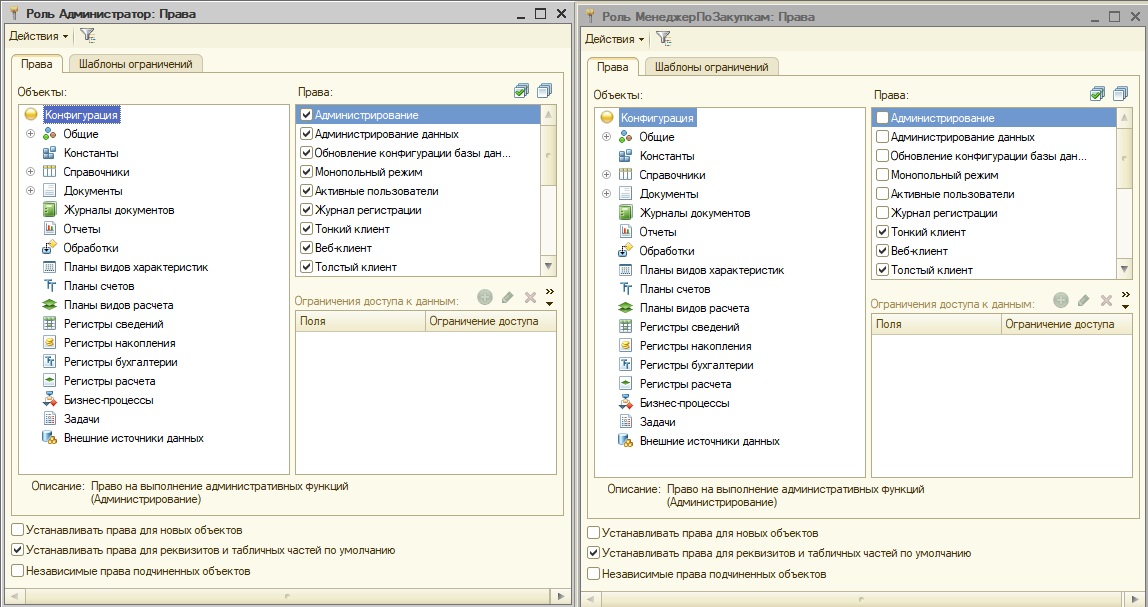
\includegraphics[width=\linewidth]{roles}
    \caption{Роли}
    \label{fig:roles}
\end{figure}

Запустим систему в режиме предприятия (рисунок \ref{fig:facility}):
\begin{figure}[H]
    \centering
    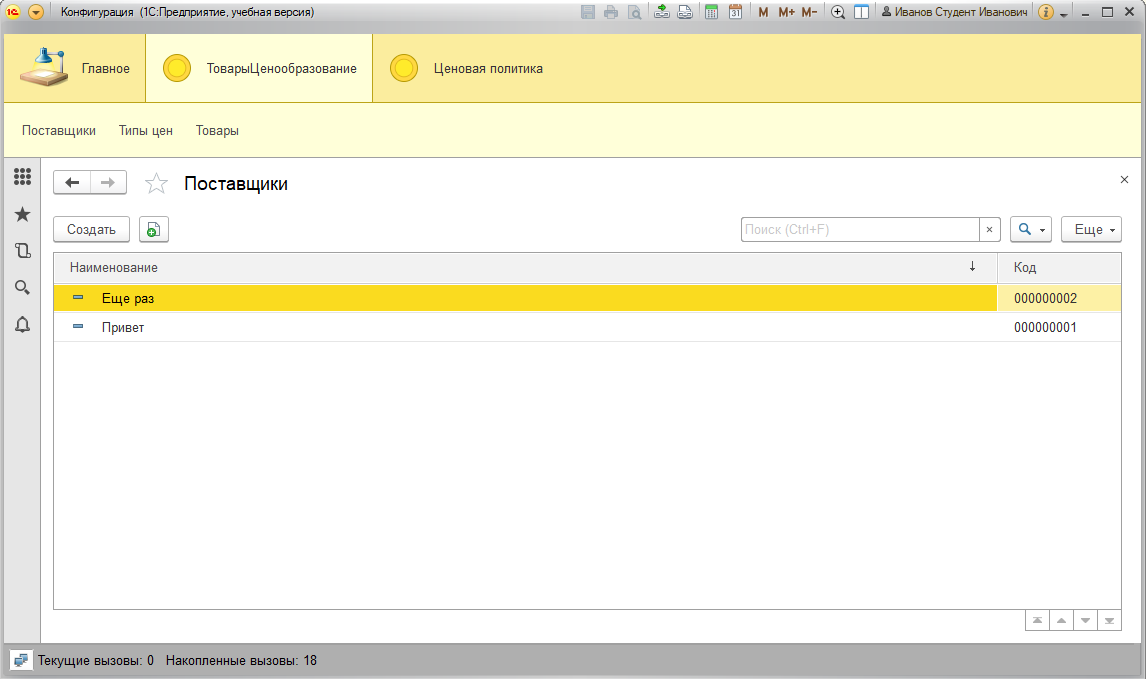
\includegraphics[width=\linewidth]{facility}
    \caption{Запуск в режиме \enquote{Предприятие}}
    \label{fig:facility}
\end{figure}

Зададим в журнале регистрации регистрацию всех событий (рисунок
\ref{fig:journal}):
\begin{figure}[H]
    \centering
    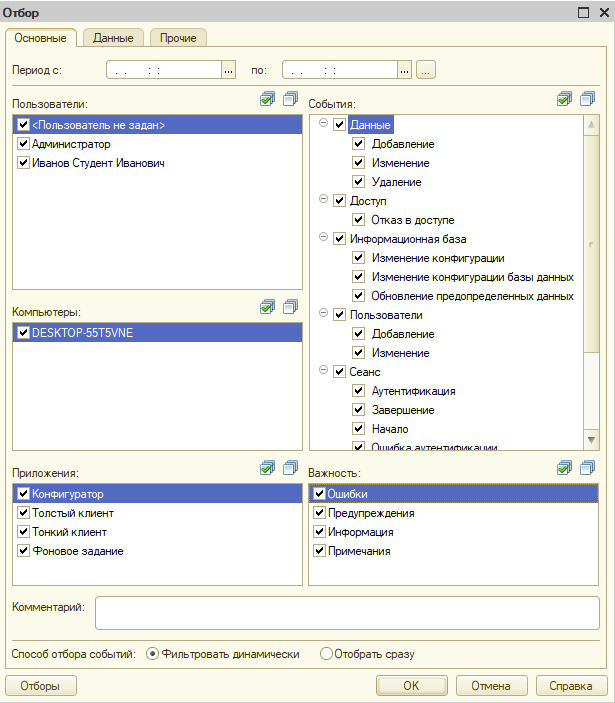
\includegraphics[width=0.6\linewidth]{journal}
    \caption{Журнал регистрации}
    \label{fig:journal}
\end{figure}

\section*{Выводы}
В ходе лабораторной работы были изучены основные компоненты имформационной базы,
такие как подсистемы, документы, справочники. Доступ к компонентам
ограничивается ролями. Конфигурировать предприятие может только пользователь с
администратиорской ролью.

Для всех компонентов, заданных при конфигурации, автоматически создается
пользовательский интерфейс для обычных пользователей.

\end{document}